% respuesta1.tex

2. Normalice hasta la 3NF y muestre cómo es la BCNF - en caso de que ésta sea diferente a la 3NF - para la siguiente relación. Debe justificar cada paso de normalización.

Produccion\_de\_Vegetales(\underline{v\#}, sembradio, año, calidad, región, país, \underline{cip}, nombrep, \underline{fecha}, cantidad)

Produccion\_de\_Vegetales(v\#) $\rightarrow$ Produccion\_de\_Vegetales(país)

Produccion\_de\_Vegetales(v\#) $\rightarrow$ Produccion\_de\_Vegetales(sembradio)

Produccion\_de\_Vegetales(v\#) $\rightarrow$ Produccion\_de\_Vegetales(año)

Produccion\_de\_Vegetales(v\#) $\rightarrow$ Produccion\_de\_Vegetales(calidad)

Produccion\_de\_Vegetales(v\#) $\rightarrow$ Produccion\_de\_Vegetales(región)

Produccion\_de\_Vegetales(sembradio,año) $\rightarrow$ Produccion\_de\_Vegetales(calidad)

Produccion\_de\_Vegetales(región) $\rightarrow$ Produccion\_de\_Vegetales(pais)

Produccion\_de\_Vegetales(cip) $\rightarrow$ Produccion\_de\_Vegetales(nombrep)

Produccion\_de\_Vegetales(v\#,cip,fecha) $\rightarrow$ Produccion\_de\_Vegetales(cantidad)


\subsection*{1NF}
Ya se encuentra en 1NF ya que todos los atributos de la relación contienen valores atómicos.

\begin{figure}[H]
	\centering
	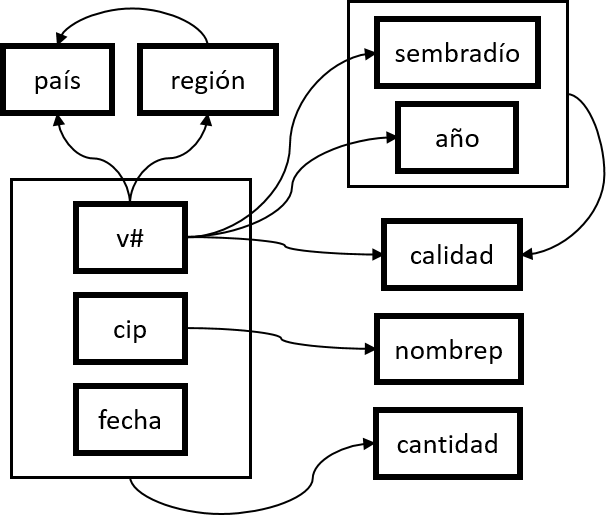
\includegraphics[scale=0.8]{img/1_1nf.png}
\end{figure}

\newpage
\subsection*{2NF}
Tenemos que sembradio, año, calidad, región, país, y nombrep no dependen totalmente de la clave primaria, por lo que procedemos a separar la relación, y tendríamos:

Almacen(\underline{v\#}, \underline{cip}, \underline{fecha}, cantidad)

Produccion(\underline{v\#}, sembradio, año, calidad, region, pais)

Nombres(\underline{cip}, nombrep)

\begin{figure}[H]
	\centering 
	\begin{overpic}[scale=0.56,]{img/2nf_almacen.png}
		\put (35, 65) {\textbf{Almacen}}
	\end{overpic}
	\hspace{0.4cm} \vrule \hspace{0.4cm}
	\begin{overpic}[scale=0.56,]{img/2nf_produccion.png}
		\put (40, 65) {\textbf{Producción}}
	\end{overpic}
	\hspace{0.4cm} \vrule \hspace{0.4cm}
	\begin{overpic}[scale=0.56,]{img/2nf_nombres.png}
		\put (35, 35) {\textbf{Nombres}}
	\end{overpic}
\end{figure}


\subsection*{3NF}
Tenemos que calidad y pais no dependen solo de la clave primaria y tienen dependencias funcionales transitivas, y esto viola la 3NF, por lo que pasamos estos atributos a otras relaciones:

Almacen(\underline{v\#}, \underline{cip}, \underline{fecha}, cantidad)

Produccion(\underline{v\#}, sembradio, año, región)

Siembra(\underline{sembradio}, \underline{año}, calidad)

Lugar(\underline{región}, país)

Nombre(\underline{cip}, nombrep)

\vspace{0.40cm}
\begin{figure}[H]
	\centering 
	\begin{overpic}[scale=0.60,]{img/2nf_almacen.png}
		\put (35, 65) {\textbf{Almacen}}
	\end{overpic}
	\hspace{0.4cm} \vrule \hspace{0.4cm}
	\begin{overpic}[scale=0.60,]{img/1-3nf_produccion.png}
		\put (40, 74) {\textbf{Producción}}
	\end{overpic}
	\hspace{0.4cm} \vrule \hspace{0.4cm}
	\begin{overpic}[scale=0.56,]{img/1-3nf_siembra.png}
		\put (35, 52) {\textbf{Siembra}}
	\end{overpic}
\end{figure}

\hrule
\vspace{0.40cm} 
\begin{figure}[H]
	\centering 
	\begin{overpic}[scale=0.60,]{img/1-3nf_lugar.png}
		\put (35, 30) {\textbf{Lugar}}
	\end{overpic}
	\hspace{0.4cm} \vrule \hspace{0.4cm}
	\begin{overpic}[scale=0.60,]{img/2nf_nombres.png}
		\put (40, 30) {\textbf{Nombre}}
	\end{overpic}
\end{figure}

\subsection*{BCNF}
Como ningún atributo no clave es determinante, tenemos que nuestras relaciones se encuentran en BCNF.